\documentclass[../main.tex]{subfiles}
\begin{document}
\chapter{Sturm-Liouville Problems}
\section{Operators and Self-Adjoint Maps}
\begin{remark}[Recap]
  Recall from IA Vectors and Matrices that a linear map $A: V_N \to V_N$ is called \textit{Hermitian} if:
  \[
    \vec{x} \cdot A \vec{y} = (A \vec{x}) \cdot \vec{y}
  \]
  or equivalently $A = A^{\dag}$.
  We also defined the standard inner product on $\C$ as:
  \[
    (\vec{x}, \vec{y}) = \sum_{i = 1}^{n} x_i \overline{y_i}
  \]

  We saw that Hermitian maps have the following properties:
  \begin{enumerate}
    \item Their eigenvalues are all real
    \item Eigenvectors corresponding to different eigenvalues are orthogonal with respect to the inner product $(\cdot, \cdot)$.
    \item There exists a set $\{\vec{y}_n\}^{N}_{n = 1}$ of eigenvectors such that every $\vec{x} \in V_N$ can be written as:
      \[
        \vec{x} = \sum_{n = 1}^{N} \hat{x}_n \vec{y}_n \text{ where } \hat{x}_n = \frac{\vec{x} \cdot \vec{y}_n}{\norm{\vec{y}_n}^2}
      \]
  \end{enumerate}
\end{remark}
Can we generalise this idea to vector spaces of functions?

Let $V$ be a vector space which is a subspace of $C^2([a, b])$ and define the inner product:
\[
  \langle f, g \rangle_{w} = \int_{a}^{b} f(x) \overline{g(x)} w(x) \d{x}
\]
where $w(x)$ is real and $w(x) > 0$ on $(a, b)$.
\begin{remark}[Notation]
  When $w \equiv 1$, we write $\langle f, g \rangle \equiv \langle f, g \rangle_{1}$.
\end{remark}

We then define the norm as usual:
\[
  \norm{f}_{w} = \sqrt{\langle f, f \rangle_{w}}
\]
\begin{definition}[Self-Adjoint Operator]
  We say that a linear operator $\mathcal{L}$ on $V$ is called \textit{self-adjoint} on the inner product space $(V, \langle \cdot, \cdot \rangle_{w})$ if:
  \[
    \langle \mathcal{L}y_1, y_2 \rangle_{w} = \langle y_1, \mathcal{L}y_2 \rangle_{w}\ \forall y_1, y_2 \in V
  \]
\end{definition}
\begin{definition}[Eigenvalue and Eigenfunction]
  For a linear operator $\mathcal{L}$ on $V$, we say that $(\lambda, y) \in \C \times (V \setminus \{0\})$ is an eigenvalue-eigenfunction pair for $\mathcal{L}$ if $\mathcal{L} y = \lambda y$.
\end{definition}
\begin{proposition}
  If $\mathcal{L}$ is self adjoint on $(V, \langle \cdot, \cdot \rangle_{w})$, then we have the following: \label{selfAdjProp}
  \begin{enumerate}
    \item The eigenvalues of $\mathcal{L}$ are real
    \item Eigenfunctions corresponding to different eigenvalues are orthogonal with respect to $\langle \cdot, \cdot \rangle_{w}$
    \item There exists a set $\{y_n\}^{n = 1}_{\infty}$ of eigenfunctions such that every $f \in V$ can be written as:
      \[
        f(x) = \sum_{n = 1}^{\infty} \hat{f}_n y_n(x) \text{ where } \hat{f}_n = \frac{\langle f, y_n \rangle_{w}}{\norm{y_n}^2_w}
      \]
  \end{enumerate}
\end{proposition}
\begin{proof}[\textbf{i}]
  Let $y$ be an eigenfunction with eigenvalue $\lambda$, that is, $y \neq 0$ and satisfies $\mathcal{L}y = \lambda y$.

  We want to show that $\lambda - \overline{\lambda} = 0$ and know that $\norm{y}^2_{w}$ is non-zero and so we consider their product:
  \begin{align*}
    (\lambda - \overline{\lambda})\norm{y}^2_w &= (\lambda - \overline{\lambda})\langle y, y \rangle_{w} \\
                                               &= \langle \lambda y, y \rangle_{w} - \langle y, \lambda y \rangle_{w} \\
                                               &= \langle \mathcal{L}y, y \rangle_{w} - \langle y, \mathcal{L}y \rangle_{w} \\
                                               &= 0
  \end{align*}
  and so $\lambda = \overline{\lambda} \implies \lambda \in \R$.
\end{proof}
\begin{proof}[\textbf{ii}]
  So we have $y_1, y_2 \neq 0$ such that $\mathcal{L}y_1 = \lambda_1 y_1$ and $\mathcal{L}y_2 = \lambda_2 y_2$ with $\lambda_1 \neq \lambda_2$.
  Appealing to a similar strategy as in \textbf{(i)}:
  \begin{align*}
    (\lambda_1 - \lambda_2) \langle y_1, y_2 \rangle_{w} &= \langle \lambda_1 y_1, y_2 \rangle_{w} - \langle y_1, \overline{\lambda_2} y_2 \rangle_{w} \\
                                                         &= \langle \lambda_1 y_1, y_2 \rangle_{w} - \langle y_1, \lambda_2 y_2 \rangle_{w} \text{ as $\lambda_2 \in \R$ by \textbf{(i)}} \\
                                                         &= \langle \mathcal{L} y_1, y_2 \rangle_{w} - \langle y_1, \mathcal{L} y_2 \rangle_{w} \\
                                                         &= 0 \text{ as $\mathcal{L}$ is self-adjoint}
  \end{align*}
  Thus $\langle y_1, y_2 \rangle_{w} = 0$.
\end{proof}
\begin{proof}[\textbf{iii}]
  Not lectured -- See II Functional Analysis.
\end{proof}
\section{Self-Adjointness and Boundary Conditions}
We wish to study problems of the form:
\begin{equation}
  \begin{cases}
  \mathcal{L}y = \lambda y & \text{ if } a < x < b \\
  \text{Boundary conditions} & \text{ at } x = a = b
  \end{cases} \label{generalForm}
\end{equation}
where $\mathcal{L}$ is a special type of differential operator, called a \textit{Sturm-Liouville} operator.
\begin{definition}[Sturm-Liouville operator]
  A \textit{Sturm-Liouville operator} is a second-order differential operator of the form:
  \[
    \mathcal{L} \argdot = \frac{1}{w}\left[-\deriv{}{x}\left(p \deriv{}{x} \argdot\right) + q \argdot\right]
  \]
  where $p, q$ and $w$ are real valued functions and $p, w > 0$ on $(a, b)$.
  We call $w$ the \textit{weight function} associated with $\mathcal{L}$
\end{definition}
What are the eigenfunctions of this operator?
$\mathcal{L} y = \lambda y$ becomes:
\[
  -\deriv{}{x}\left[p \deriv{y}{x}\right] + qy = \lambda w y \text{ for } a < x < b
\]
We then impose the boundary conditions in \cref{generalForm} by forcing $y$ to belong to some vector space $V$ that enforces them.
Thus \cref{generalForm} becomes:
\[
  Ly = \lambda y,\ y \in V
\]
\begin{definition}[Singular and non-singular endpoints]
  Given a Sturm-Liouville operator on $(a, b)$, we say that an endpoint $c \in \{a, b\}$ is \textit{singular} if $p(c) = 0$ and say that it is \textit{non-singular} otherwise.
\end{definition}
We will only specify boundary conditions at non-singular endpoints.
At such endpoints $c$ will impose \textit{real homogeneous} boundary conditions of the form:
\[
  \alpha_c y(c) + \beta_c y'(c) = 0
\]
where $\alpha_c, \beta_c \in \R$ and $\alpha^2_c + \beta^2_c \neq 0$ (i.e. they are not both zero).
Note that if $y_1, y_2$ satisfy boundary conditions of this forms then so does $c_1 y_1 + c_2 y_2$ for any constants $c_1$ and $c_2$.

So given a Sturm-Liouville operator we enforce boundary conditions by working on a vector space of form:
\[
  V = \{y \in C^2[a, b]: y \text{ satisfies real homogeneous B.C.s at each non-singular endpoint }\}
\]
\begin{example}
  Consider the vector space:
  \[
    V = \{y \in C^2[0, \pi]: y(0) = 0\}
  \]
  for the problem:
  \[
    -\deriv{}{x}\left[\cos\left(\frac{x}{2}\right) \deriv{y}{x}\right] + \sin\left(\frac{x}{2}\right)y = \lambda y
  \]
  The above is $\mathcal{L} y = \lambda y$ for a Sturm-Liouville operator with $p = \cos\left(x/2\right)$, $q = \sin(x/2)$ and $w \equiv 1$.

  We see that $p(\pi) = 0$ and $p(0) \neq 0$, that is $\pi$ is singular and $0$ is non-singular.
  This is consistent with the homogeneous real boundary conditions enforced by $V$.
\end{example}
\begin{remark}[Recap]
  Recall that the \textit{Wronskian} from IA Differential Equations was defined as:
  \[
    W(f, g) = fg' - f'g
  \]
\end{remark}
We now equip $V$ with the inner product $\langle \cdot, \cdot \rangle_{w}$ where $w$ is the weight function associated with $\mathcal{L}$, allowing us to use the properties in \cref{selfAdjProp}.
\begin{proposition}
  If $V$ is a vector space associated with Sturm-Liouville operator $\mathcal{L}$, then $\mathcal{L}$ is self-adjoint on ($V, \langle \cdot, \cdot \rangle_{w}$) where $w$ is the weight function corresponding to $\mathcal{L}$.
\end{proposition}
\begin{proof}
  We want to show that $\langle \mathcal{L}y_1, y_2 \rangle_{w} = \langle y_1, \mathcal{L}y_2 \rangle_{w}$ for all $y_1, y_2 \in V$.

  For any $y_1, y_2 \in C^2[a, b]$, we have:
  \begin{align*}
    \langle \mathcal{L}y_1, y_2 \rangle_{w} - \langle y_1, \mathcal{L}y_2 \rangle_{w} &= \int_{a}^{b} \frac{1}{w}[-(py_1')' + qy_1]\overline{y_2} w\d{x} - \int_{a}^{b} \frac{1}{w} y_1[-(p \overline{y_2}')' + q \overline{y_2}]w \d{x} \\
                                                                                      &= \int_{a}^{b} [y_1(p \overline{y_2}')' - \overline{y_2}(p y_1')'] \d{x} \\
                                                                                      &= \int_{a}^{b} [y_1 p' \overline{y_2}' + y_1 p \overline{y_2}'' - \overline{y_2} p' y_1' - \overline{y_2} p y_1''] \d{x} \\
                                                                                      &= \int_{a}^{b} [p'(y_1 \overline{y_2}' - y_1'\overline{y_2}) + p(y_1 \overline{y_2}'' - y_1'' \overline{y_2})] \d{x} \\
                                                                                      &= \int_{a}^{b} [p(y_1 \overline{y_2}' - y_1' \overline{y_2})]' \d{x} \\
                                                                                      &= p(x) W(y_1, \overline{y_2})(x)
  \end{align*}
  Now assume that $y_1, y_2 \in V$.
  If $c \in \{a, b\}$ is singular then $p(c) = 0$, so $p(c) W(y_1, \overline{y_2})(c) = 0$.
  Otherwise, if $c$ is non-singular, then because $y_1, y_2 \in V$, they obey boundary conditions of the form:
  \[
    \alpha_c y(c) + \beta_c y'(c) = 0
  \]
  where $\alpha_c, \beta_c \in \R$ and $\alpha_c^2 + \beta_c^2 = 0$.
  Since $\alpha_c, \beta_c \in \R$, the same boundary conditions hold for $\overline{y}$ by taking the complex conjugate.

  So we therefore have:
  \[
    \begin{pmatrix}
    y_1(c) & y_1'(c) \\
    \overline{y_2}(c) & \overline{y_2}'(c) \\
    \end{pmatrix} \begin{pmatrix}
    \alpha_c \\
    \beta_c \\
    \end{pmatrix} = \vec{0}
  \]
  But since $(\alpha_c, \beta_c)^{\trans} \neq \vec{0}$, this matrix has non-trivial kernel and so has determinant 0:
  \[
    0 = \begin{vmatrix}
    y_1(c) & y_1'(c) \\
    \overline{y_2}(c) & \overline{y_2}'(c) \\
    \end{vmatrix} = W(y_1, \overline{y_2})(c)
  \]
  So at non-singular endpoints $c \in \{a, b\}$, we also have $p(c) W(y_1, \overline{y_2})(c) = 0$.

  Hence if $y_1, y_2 \in V$, then:
  \[
    \langle \mathcal{L}y_1, y_2 \rangle_{w} - \langle y_1, \mathcal{L}y_2 \rangle_{w} = 0
  \]
  that is, $\mathcal{L}$ is self adjoint on $(V, \langle \cdot, \cdot \rangle_{w})$.
\end{proof}
\section{Solving Sturm-Liouville Problems}
\begin{remark}[Recap]
  Recall from IA Vectors and Matrices that if $A$ is hermitian then we can always pick its eigenvectors to be real.
\end{remark}
Since we know that $\mathcal{L}$ is self adjoint on $(V, \langle \cdot, \cdot \rangle_{w})$, by \cref{selfAdjProp} \textbf{(i)}, we know that all the eigenvalues are real.
Suppose that we have a complex valued function $f \in V$.
We can express it as $f = u + iv$ for real valued $u$ and $v$.
If $f$ is an eigenfunction, then since $p, q, w, \lambda \in \R$, we have:
\[
  \lambda u + i\lambda v = \lambda f = \mathcal{L} f = \mathcal{L} u + i\mathcal{L} v \implies \mathcal{L} u = \lambda u,\ \mathcal{L} v = \lambda v
\]
so we can always pick our eigenfunctions to be real.
Thus without loss in generality, we assume that all of our eigenfunctions are real valued.

So for $f \in V$ and $y$ an eigenfunction of $\mathcal{L}$, then we can drop the complex conjugate from the inner product:
\[
  \langle f, y \rangle_{w} = \int_{a}^{b} f(x) y(x) w(x) \d{x}
\]
From \cref{selfAdjProp} \textbf{(ii)} and \textbf{(iii)}, we know that there exists $(\lambda_n, y_N)_{n = 1}^\infty \in \R \times (V \setminus \{0\})$ such that $L y_n = \lambda_n y_n$ with the property that if $\lambda_n \neq \lambda_m$, then:
\[
  \langle y_n, y_m \rangle_{w} = \int_{a}^{b} y_n(x) y_m(x) w(x) \d{x} = 0
\]
and for any $f \in V$, we can write:
\[
  f(x) = \sum_{n = 1}^{\infty} \hat{f}_n y_n(x) \text{ where } \hat{f}_n = \frac{\langle f, y_n \rangle_{w}}{\norm{y_n}^2_{w}}
\]
It will turn out that for the Sturm-Liouville problems will will study, that our eigenvalues are bounded below and can be ordered so that $\lambda_1 < \lambda_2 < \lambda_3 < \cdots$ with $\lambda_n \to \infty$ as $n \to \infty$.
\begin{example}
  Consider the problem:
  \[
    \begin{cases}
    -y'' = \lambda y & \text{ if } 0 < x < L \\
    y(0) = 0 &  \\
    y(L) = 0 &
    \end{cases}
  \]
  This is a Sturm-Liouville eigenvalue problem with $p = 1$, $q = 0$, $w = 1$ on the set:
  \[
    V = \{y \in C^2[0, L]: y(0) = y(L) = 0\}
  \]
  We now solve the differential equation $y'' + \lambda y = 0$.
  In the case of $\lambda < 0$, then after applying the boundary conditions, we see that all solutions are trivial so we require $\lambda \geq 0$ for non-trivial solutions.

  In this case, the general solution is:
  \[
    y = A \sin(\sqrt{\lambda} x) + B \cos(\sqrt{\lambda} x)
  \]
  We then see that $y(0) = 0 \implies B = 0$ and $y(L) = 0$ tells us that:
  \[
    A \sin (\sqrt{\lambda} L) = 0 \iff L\sqrt{\lambda} = n \pi \text{ for } n \in \N_0
  \]
  So the eigenvalue-eigenfunction pairs are:
  \[
    \lambda_n = \left(\frac{\pi n}{L}\right)^2,\ y_n(x) = \sin\left(\frac{n\pi x}{L}\right) \text{ for } n \in \N_0
  \]
  We can verify that indeed:
  \[
    \int_{0}^{L} y_n(x) y_m(x) \d{x} = \frac{L}{2} \delta_{n m}
  \]
  We also obtain that for any $f \in V$, we can write:
  \[
    f(x) = \sum_{n=0}^{\infty} \hat{f}_n \sin\left(\frac{n \pi x}{L}\right)
  \]
  where:
  \[
    \hat{f}_n = \frac{\langle f, y_n \rangle_{w}}{\norm{y_n}_{w}^2} = \frac{2}{L} \int_{0}^{L} f(x) \sin\left(\frac{n \pi x}{L}\right) \d{x}
  \]
  So we have re-derived the Fourier sine series for $f \in C^2([0, L])$ with $f(0) = f(L) = 0$ as defined in \cref{sinCosSeries}.
\end{example}
\section{Reduction to Sturm-Liouville Form}
Consider a generic eigenvalue problem of the form:
\begin{equation}
  \alpha(x) y'' + \beta(x) y' + \gamma(x) y + \lambda y = 0 \text{ on } a < x < b \label{genEigenval}
\end{equation}
where $\alpha(x) > 0$ on $(a, b)$.
We would like to reduce this to Sturm-Liouville form so that we can use the results established so far in this chapter.

We can do this by dividing through by $\alpha(x) > 0$ and multiplying by an integrating factor $I(x)$:
\[
  I(x) = \exp\left[- \int_{}^{x} \frac{\beta(t)}{\alpha(t)} \d{t}\right]
\]
\begin{proposition}
  The problem in \cref{genEigenVal} is equivalent to the Sturm-Liouville problem:
  \[
    -\deriv{}{x}\left[p \deriv{y}{x}\right] + qy = \lambda w y
  \]
  where:
  \[
    p(x) = I(x),\ q(x) = - \frac{\gamma(x)I(x)}{\alpha(x)} \text{ and } w(x) = \frac{I(x)}{\alpha(x)}
  \]
\end{proposition}
\begin{proof}
  We see that $p(x) > 0$ and $w(x) > 0$ on $(a, b)$ as required for a Sturm-Liouville operator $\mathcal{L}$.
  From the definition of $\mathcal{L}$, we see that:
  \begin{align*}
    w\mathcal{L}y - w\lambda y &= -\deriv{}{x}\left[p \deriv{y}{x}\right] + qy - \lambda w y \\
                             &= - p'y' - py'' + qy - \lambda w y \\
                             &= - \frac{\beta}{\alpha} Iy' - Iy'' - \frac{\gamma}{\alpha}I - \frac{\lambda}{\alpha} Iy \\
                             &= I(x) \left[-y'' - \frac{\beta}{\alpha}y' - \frac{\gamma}{\alpha} y - \frac{\lambda}{\alpha}\right]
  \end{align*}
  Since $I(x) > 0$, this right hand side vanishes if and only if \cref{genEigenval} vanishes and so if and only if $\mathcal{L} y = \lambda y$ since $w(x) > 0$.
\end{proof}
\begin{example}
  Consider the eigenvalue problem:
  \[
    \begin{cases}
    y'' - 2y' + \lambda y = 0 & \text{ if } 0 < x < 1 \\
    y(0) = 0 &  \\
    y'(1) = 0 &
    \end{cases}
  \]
  The integrating factor for this is:
  \[
    I(x) = \exp\left[\int_{}^{x} (-2) \d{x}\right] = e^{-2x}
  \]
  so $p = e^{-2x}, q = 0, w = e^{-2x}$, i.e. the problem is equivalent to:
  \[
    \mathcal{L} y = -\deriv{}{x}\left[e^{-2x} \deriv{y}{x}\right] = \lambda e^{-2x} y
  \]

  The general solution to the original problem is:
  \[
    y = e^{x}[A \sinh(\sqrt{1 - \lambda} x) + B \cosh(\sqrt{1 - \lambda}x)]
  \]
  for $\lambda \in \R$.

  In the case of $1 - \lambda \geq 0$, we get only trivial solutions after applying the boundary conditions.
  Thus to look for eigenvalues we set $1 - \lambda = -\mu^2$, where without loss in generality $\mu > 0$.
  In this case we can write the general solution as:
  \[
    y = e^{x}[A \sin(\mu x) + B \cos(\mu x)]
  \]
  Applying the boundary conditions, $y(0) = 0 \implies B = 0$ and $y'(1) = 0$ gives:
  \[
    0 = A e [\sin \mu + \mu \cos \mu]
  \]
  So for non-trivial solutions we need the bracketed term to vanish, i.e.:
  \[
    \tan \mu = - \mu \text{ for } \mu > 0
  \]
  The solutions to these are precisely the intersections between the graphs of $\tan \mu$ and $-\mu$:
  \begin{center}
  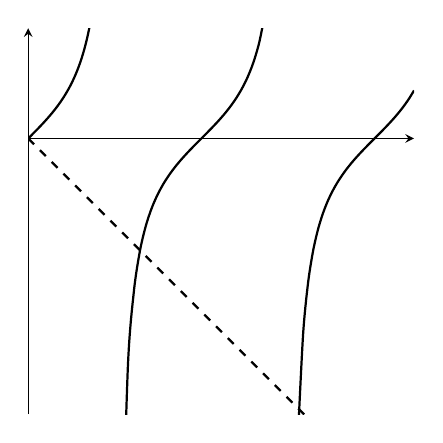
\begin{tikzpicture}[>=stealth, scale=0.7]
    \draw[->] (0, 0) -- (7, 0);
    \draw[->] (0, -5) -- (0, 2);
    \clip (0, -5) rectangle (7, 2);
    \draw[thick, dashed] (0, 0) -- (7, -7);
    \draw[thick, domain=0:1.2, smooth, variable=\x] plot ({\x}, {tan(\x r)});
    \draw[thick, domain=1.7:4.3, smooth, variable=\x] plot ({\x}, {tan(\x r)});
    \draw[thick, domain=4.9:7, smooth, variable=\x] plot ({\x}, {tan(\x r)});
  \end{tikzpicture}
  \end{center}
  From this we see that we get infinitely many solutions which we can order with $\mu_1 < \mu_2 < \cdots$.
  We also see that $\mu_n \to \infty$ as $n \to \infty$.

  Thus we have infinitely many eigenvalues $\lambda_n = 1 + \mu^2_n$ with ordering $\lambda_1 < \lambda_2 < \cdots$ and $\lambda_n \to \infty$ as $n \to \infty$.

  The eigenfunctions are $y_n(x) = e^{x}\sin(\mu_n x)$ which we expect to be orthogonal with respect to a suitable inner product.
  We saw that $w = e^{-2x}$ and so we check that:
  \begin{align*}
    \langle y_n, y_m \rangle_{w} &= \int_{0}^{1} e^{x} \sin(\mu_n x) \cdot e^{x} \sin(\mu_n x) \cdot e^{-2x} \d{x} \\
                                 &= \int_{0}^{1} \sin(\mu_n x) \sin(\mu_m x) \d{x} \\
                                 &= \frac{1}{2} \int_{0}^{1} [\cos[(\mu_n - \mu_m)x] - \cos[(\mu_n + \mu_m)x]] \d{x} \\
                                 &= \frac{1}{2}\left[\frac{\sin(\mu_n - \mu_m)}{\mu_n - \mu_m} - \frac{\sin(\mu_n + \mu_m)}{\mu_n + \mu_m}\right] \\
                                 &= \frac{1}{2}\left[\frac{\sin \mu_n \cos \mu_m - \sin \mu_m \cos \mu_n}{\mu_n - \mu_m} - \left(\frac{\sin \mu_n \cos \mu_m + \sin \mu_m \cos \mu_n}{\mu_n + \mu_m}\right)\right] \\
                                 &= \frac{1}{2} \cos \mu_n \cos \mu_m \left[\frac{\tan \mu_n - \tan \mu_m}{\mu_n - \mu_m} - \left(\frac{\tan \mu_n + \tan \mu_m}{\mu_n + \mu_n}\right)\right] \\
                                 &= \frac{1}{2} \cos \mu_n \cos \mu_m \left[\frac{-\mu_n + \mu_m}{\mu_n - \mu_m} + \frac{\mu_n + \mu_m}{\mu_n + \mu_m}\right] \\
                                 &= \frac{1}{2} \cos \mu_n \cos \mu_m[-1 + 1] \\
                                 &= 0
  \end{align*}
\end{example}
\begin{remark}
  The process of checking that functions are orthogonal can be quite tedious.
  It is therefore usually quicker to construct a Sturm-Liouville problem of which they are eigenfunctions and then appeal to Sturm-Liouville theory to conclude.
\end{remark}
\end{document}
